\documentclass[a4paper]{coursepaper-br}

\usepackage{ucs}
\usepackage[utf8x]{inputenc}
\usepackage[brazil]{babel}
\usepackage[T1]{fontenc}
\usepackage{SIunits}
\usepackage{ae,aecompl}
\usepackage{graphicx}
\usepackage{listings}
\usepackage{enumitem}
\usepackage{subfig}
\usepackage{a4wide}

\hyphenation{sub-re-gi-ões}

\title{Implementação de um algoritmo de rastreamento de objetos móveis em vídeo}
\author{João Felipe Santos}
\college{Universidade Federal de Santa Catarina \\
Centro Tecnológico \\ 
Departamento de Engenharia Elétrica}
\coursename{Projeto Nível I em Controle e Processamento de Sinais I}
\coursenumber{EEL7815 - }
\studentnumber{05141273}
\instructor{Joceli Mayer, Ph.D.}
\date{01 de julho de 2010}

\begin{document}
\maketitle
 
\section{Introdução}

O problema de rastreamento de objetos em vídeo é considerado
importante atualmente, especialmente ao se considerar suas aplicações
em visão computacional e análise automática de vídeos. Este problema
pode ser dividido basicamente em três partes \cite{Yilmaz2006}:

\begin{itemize}
 \item Detecção de objetos de interesse em movimento 
 \item Rastreamento destes objetos quadro a quadro
 \item Análise da trajetória dos objetos para reconhecimento de seu
   comportamento
\end{itemize}

Como áreas de aplicação, pode-se citar o monitoramento de segurança
automático, reconhecimento de gestos, auxílio a navegação de veículos
e detecção automática de objetos baseada em seu padrão de movimento.

Este procedimento pode ser feito em diversos níveis de complexidade e
refinamento. Para certas aplicações, é importante que o processamento
possa ser realizado em tempo real, isto é, há um tempo relativamente
curto para o processamento de um novo quadro a partir do momento em
que ele foi adquirido. É importante levar em consideração o
compromisso entre as funcionalidades do algoritmo e sua complexidade.

O algoritmo proposto neste trabalho visa o rastreamento de pessoas em
vídeos de monitoramento de segurança. Para detecção de objetos de
interesse em um quadro, é utilizado um extrator de características
chamado SURF (\emph{Speeded-Up Robust Features}), e para localização
destes objetos a cada quadro, é feita uma busca multidimensional. Pelo
fato de ambos os algoritmos serem complexos computacionalmente, a
ideia básica deste trabalho é setorizar a região de busca para que a
quantidade de pixels a serem processados por quadro seja menor do que
a imagem inteira.

O restante do relatório está organizado da seguinte forma: as seções
\ref{sec:featdet} e \ref{sec:objtrack} detalham melhor os
procedimentos de extração de características e rastreamento utilizados
e traçam rapidamente um paralelo entre outras técnicas. A seção
\ref{sec:impl} mostra detalhes de implementação, incluindo a estrutura
do algoritmo e o ambiente computacional utilizado para programação. A
seguir são descritos os resultados obtidos, elaboradas algumas
considerações finais sobre os resultados e os principais problemas
encontrados.

\section{Extração de características}
\label{sec:featdet}

A extração de características de uma imagem busca detectar pontos ou
formas de interesse que possam ser utilizados para rastreamento ou
reconhecimento. Existe um grande número de propostas na literatura
para este fim, baseando-se em características da imagem como cor,
textura, bordas ou cantos. Um detector tem como principal
característica a repetibilidade, isto é, é necessário que detecte
pontos semelhantes em imagens distintas. Adicionalmente, um detector
pode ser invariante a escalamento e rotação.

Após a detecção destes pontos, é necessário associar a eles
descritores, para que se possa identificá-los. O tipo de descritor
depende muito do formato de características extraído. Descritores
precisam ser robustos o bastante, para que pontos similares apresentem
descritores similares. Também é necessário que pontos muito diferentes
apresentem descritores também diferentes.

\subsection{Alguns exemplos de características}

\begin{description}
 \item[Borda] o detector Canny identifica pontos de interesse em
   bordas da imagem. A imagem original é filtrada com um filtro
   Gaussiano para redução de ruído. A seguir, são calculadas a
   magnitude e o ângulo dos gradientes da imagem. Então, são
   suprimidos os valores não-máximos dos gradientes, de modo que
   restem somente as bordas afinadas, que são analisadas e conectadas
   \cite{Gonzalez2007}. Este algoritmo é somente um detector, sendo
   necessário algum método para geração de descritores a partir das
   bordas detectadas. A figura \ref{fig:canny} mostra um exemplo de
   imagem processada com esse detector.
 \item[Cantos/curvaturas] alguns detectores/descritores, como Harris,
   detectam locais com alta curvatura, que podem ou não ser cantos de
   objetos. A figura \ref{fig:harris} mostra marcações de pontos
   detectados com um detector Harris sobre a imagem original.
\end{description}

\begin{figure}
\centering
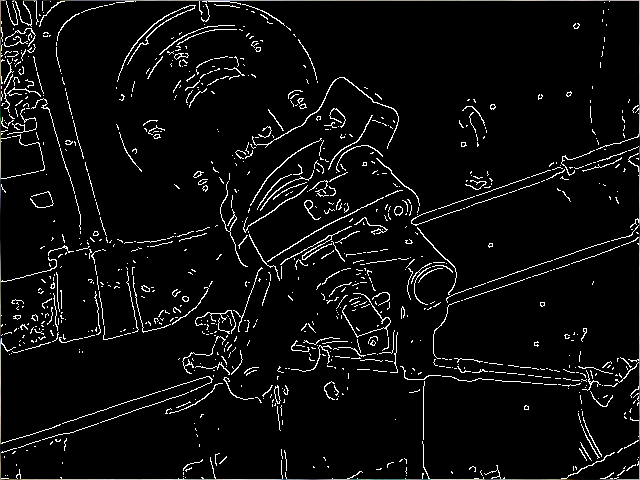
\includegraphics[width=0.5\textwidth]{Valve_monochrome_canny_(6).PNG}
\caption{Imagem processada com o detector de bordas Canny}
\label{fig:canny}
\end{figure}

\begin{figure}
\centering
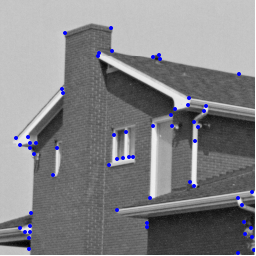
\includegraphics[width=0.5\textwidth]{HarrisHouseTest.png}
\caption{Pontos de interesse encontrados pelo detector Harris}
\label{fig:harris}
\end{figure}

\subsection{SURF - Speeded Up Robust Features}

O algoritmo utilizado neste trabalho para extração de características
foi o SURF \cite{Bay2008}. Este algoritmo é invariante a escalamento e
rotação, e utiliza-se de alguns recursos para redução de complexidade
computacional. Esta seção dá uma ideia geral de seu funcionamento,
para maior detalhamento recomenda-se a leitura do artigo original.

O detector de pontos de interesse do SURF é baseado em uma aproximação
da matriz Hessiana, calculada para cada ponto da imagem. Os pontos de
interesse encontrados são estruturas do tipo \emph{blob}, que ocorrem
nas regiões onde o determinante da matriz é máximo. O cálculo desta
matriz é baseado na convolução da imagem em escala de cinza com a
derivada parcial de segunda ordem de uma Gaussiana truncada. É
possível definir um nível de detecção para o algoritmo baseado em um
valor mínimo do determinante, o que resulta na diminuição da
quantidade de pontos encontrados. No entanto, percebe-se que pontos
com o determinante mais elevado são mais robustos. A figura
\ref{fig:hessian} mostra, respectivamente, a detecção de pontos com
determinante maior que 500, 1000 e 3000.

\begin{figure}
 \centering
 \subfloat[]{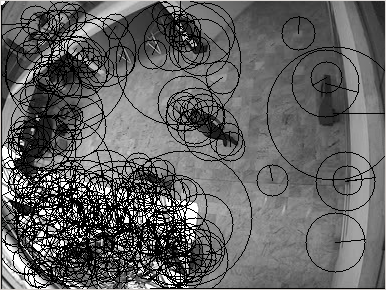
\includegraphics[width=0.3\textwidth]{hessian500.png}}
 \subfloat[]{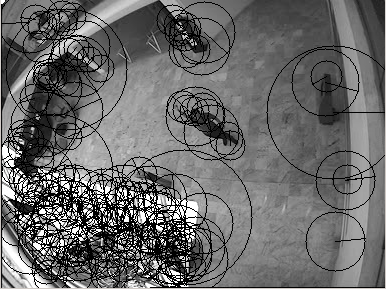
\includegraphics[width=0.3\textwidth]{hessian1000.png}}
 \subfloat[]{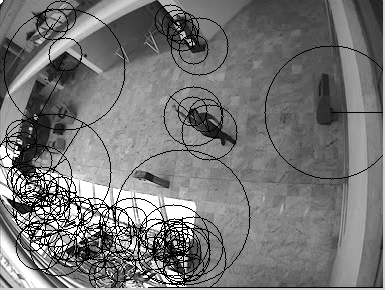
\includegraphics[width=0.3\textwidth]{hessian3000.png}}
 \caption{Pontos de interesse com determinante maior que 500, 1000 e
   3000 (da esquerda para a direita)}
 \label{fig:hessian}
\end{figure}

A detecção de pontos se dá em diferentes escalas. Para evitar os
problemas associados ao \emph{downsampling}, ao invés de reduzir a
imagem iterativamente, a máscara do filtro é aumentada. O espaço de
escalamentos é dividido em oitavas, cada uma representando a
convolução da saída do filtro inicial com filtros aumentados em
escalas intermediárias. Para o algoritmo implementado, foram usadas 3
oitavas. Na figura \ref{fig:hessian}, o tamanho dos círculos
representa a escala onde a característica foi detectada, e o eixo
representa a direção.

Os descritores são baseados na soma das respostas wavelet de
Haar. Fundamentalmente, os descritores representam a distribuição
espacial dos gradientes na região de interesse. Cada região é dividida
em subregiões $4 \times 4$, e para cada divisão da subregião são calculadas
respostas wavelet Haar na horizontal e na vertical. Os descritores
resultantes são a soma das respostas e de seus módulos na horizontal e
na vertical ($\sum dx, \sum dy, \sum |dx|, \sum |dy|$). Desta forma,
cada descritor é um vetor com 64 coeficientes. Uma variação do
algoritmo possibilita obter descritores com 128 coeficientes, que é
mais distintivo mas por ter dimensões maiores tornaria o processo de
busca mais lento.

\section{Rastreamento de objetos}
\label{sec:objtrack}

O rastreamento de objetos visa determinar a posição e o deslocamento
de objetos em uma sequência de quadros. Para rastreamento de
movimento, existem métodos baseados em busca de descritores e
métodos baseados em fluxo óptico.

Métodos baseados em fluxo óptico são capazes de identificar regiões em
movimento, sem detectar objetos propriamente ditos. Este fato evita a
necessidade das operações de busca multidimensional em um espaço de
descritores. O algoritmo de Lucas-Kanade \cite{Bradski2008}, um método
deste tipo, considera as propriedades de brilho constante,
persistência temporal e coerência espacial e, com isso, faz uma
estimativa de vetores de velocidade a partir do movimento de pixels em
regiões selecionadas.

Os algoritmos baseados em busca de descritores determinam um modelo
para o objeto a ser rastreado baseado nos descritores que podem ser
extraídos de uma imagem inicial. A partir deste modelo, é possível
fazer buscas por descritores próximos aos do modelo nos descritores
encontrados em quadros subsequentes. Caso o descritor seja
suficientemente robusto e a imagem não tenha sofrido alterações
bruscas, há grande probabilidade de o conjunto de descritores mais
próximo, encontrado em um outro quadro, ainda represente o mesmo
objeto.

O rastreamento baseado em descritores pode apresentar grande
complexidade computacional caso seja necessário extrair descritores e
fazer uma busca em um espaço multidimensional com muitos pontos para
cada quadro. Por conta disso, os métodos em geral apresentam alguma
maneira de modelar a trajetória do objeto rastreado e reduzir a área
da imagem na qual a busca deve ser realizada \cite{Zhou2009}. Esta
foi a estratégia adotada para o algoritmo implementado.

\section{Implementação}
\label{sec:impl}

Esta seção discute algumas características da aplicação implementada
e escolhas de projeto.

\subsection{Ambiente de programação}

Como ambiente de programação para desenvolvimento rápido, foi
utilizada a linguagem de programação Python \cite{python}. Esta é uma
linguagem de alto nível multiparadigma, permitindo o uso de conceitos
como programação orientada a objetos e programação funcional.

Por ser uma linguagem interpretada, seu desempenho não é o ideal para
processamento de sinais, especialmente para vídeo. Para estes casos, a
linguagem conta com uma interface para bibliotecas escritas em código
nativo de uma arquitetura, como C, C++ e FORTRAN, possibilitando unir
as facilidades de uma linguagem de alto nível interpretada (não ser
necessário compilar o programa a cada alteração, por exemplo) ao alto
desempenho de código nativo.

Para operações numéricas matriciais foi utilizada uma biblioteca para
computação científica desenvolvida para a linguagem Python, chamada
NumPy \cite{numpy}.

Para processamento de imagens, foi utilizada a biblioteca OpenCV
\cite{opencv}, em sua versão 2.1. Esta biblioteca conta com grande
variedade de funções para implementação de aplicações para visão
computacional em tempo real. Neste projeto, foram utilizadas
basicamente funções para leitura de imagens e vídeos, operações
matriciais e extração de características SURF.

Além destas, foi utilizada a biblioteca FLANN (\emph{Fast Library for
  Approximate Nearest Neighbors}) para busca por pontos vizinhos em
espaços multidimensionais \cite{flann}.

Tanto o interpretador para a linguagem Python quanto as bibliotecas e
ferramentas utilizadas são publicados sob licenças livres e estão
disponíveis na página dos respectivos projetos.

\subsection{Premissas utilizadas na implementação}

Para redução da complexidade computacional do algoritmo, visando sua
execução em tempo real, algumas premissas foram adotadas. Além disso,
algumas escolhas foram feitas para que o algoritmo possa ser utilizado
em situações gerais.

\begin{itemize}
 \item O objeto a ser rastreado encontra-se em uma região geométrica
   regular pré-determinada (na implementação, um quadrado). Somente
   descritores encontrados nesta região serão observados.
 \item Objeto move-se com velocidade relativamente baixa, de modo
   que seu deslocamento não faz com que ele saia completamente da
   região onde estava no quadro anterior.
 \item Não há um modelo do objeto definido previamente. Este modelo é
   extraído de um quadro da própria sequência.
\end{itemize}


\subsection{Estrutura geral do algoritmo}

O programa opera de acordo com a seguinte sequência de passos:

\begin{enumerate}
 \item Recebe do usuário o limiar mínimo do determinante da matriz
   Hessiana e a sequência a ser processada.
 \item Extrai as características do quadro inicial e mostra o quadro com
   marcação de características para o usuário.
 \item Recebe do usuário a região inicial a ser rastreada (coordenadas
   da origem do quadrado e tamanho em pixels) e gera uma máscara
   binária correspondente (figura \ref{fig:reference}).
 \item Para cada quadro subsequente:
\begin{enumerate}
 \item Extrai as características da seção demarcada pela máscara
   ampliada de 10\% do quadro.
 \item Caso seja o primeiro quadro, gera o índice para busca. Caso
   contrário, calcula as distâncias entre os pontos encontrados e os
   pontos indexados.
 \item Caso não seja o primeiro quadro, remove os vizinhos mais
   distantes da lista de vizinhos, isto é, a lista de vizinhos fica
   com um único vizinho para cada ponto do quadro original.
 \item Calcula o centróide dos pontos na lista de vizinhos e coloca
   este ponto como centróide da máscara da região rastreada.
 \item Marca a região rastreada no quadro e salva o quadro na
   sequência processada.
\end{enumerate}
 \item Exibe a sequência processada (figura \ref{fig:target}).
\end{enumerate}

\begin{figure}
\centering
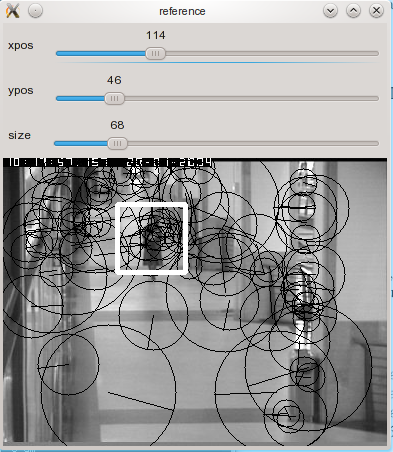
\includegraphics[width=0.5\textwidth]{reference.png}
\caption{Janela do programa para seleção da região de interesse}
\label{fig:reference}
\end{figure}

\begin{figure}
\centering
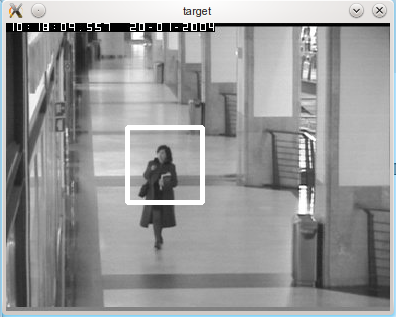
\includegraphics[width=0.5\textwidth]{target.png}
\caption{Janela do programa mostrando a sequência processada}
\label{fig:target}
\end{figure}


\section{Resultados}
\label{sec:res}

O algoritmo foi testado através de sequências de imagens de câmeras de
segurança, adquiridas no site do projeto CAVIAR \cite{Fisher2007}. As
sequências utilizadas mostram pessoas circulando em um corredor e um
hall. O objetivo foi verificar se o algoritmo era capaz de rastrear o
movimento de uma ou mais pessoas em um quadro até que as pessoas
saíssem da cena.

As sequências utilizadas foram ``Fight\_RunAway'', ``Walk2'',
``OneStopEnter1cor'' e ``TwoEnterShop1cor'', sendo os dois primeiros
gravados com uma mesma câmera na mesma posição e os dois últimos com
outra câmera em outra posição. A resolução dos vídeos é $384 \times
288$ pixels, 25 quadros por segundo (padrão PAL). Foram utilizadas as
sequências de imagens em JPEG, extraídas dos arquivos MPG previamente
para facilitar a visualização e indexação dos quadros fora da execução
do programa.

Os resultados em geral foram satisfatórios. São necessários ajustes do
valor de limiar do determinante da Hessiana para obter melhores
resultados em cada sequência, pois para rastrear pessoas que aparecem
em menor escala ou menor contraste com o cenário, é necessário obter
pontos com valor de determinante menor. A região rastreada não segue
uma trajetória suave, pois não foi utilizado nenhum método de
modelagem de trajetória do objeto.

Nas sequências ``Fight\_RunAway'' e ``Walk2'', ocorreram alguns
problemas ao rastrear as pessoas que se aproximam da região iluminada
diretamente pela janela. Pelo fato desta região possuir uma
distribuição de intensidades dos pixels diferente do modelo original,
os descritores extraídos nessa região devem ser bastante diferentes
dos originais, o que explicaria o problema obtido.

\section{Considerações finais}
\label{sec:fin}

O rastreamento de objetos em sequências de vídeo utilizando
características extraídas com o algoritmo SURF mostrou-se satisfatório
para as sequências testadas. Com as premissas assumidas para o
algoritmo, foi possível rastrear pessoas em vídeos com resolução
baixa. Existe um ruído alto na trajetória encontrada por não ter sido
realizado nenhum tipo de estimativa ``inteligente'' de trajetória.

\subsection{Problemas encontrados e possíveis melhorias}

Alguns problemas encontrados e possíveis melhorias são os seguintes:

\begin{itemize}
 \item Ruído na trajetória estimada: como já foi citado, algum tipo de
   modelagem para estimação de trajetória poderia suavizar o
   rastreamento obtido.
 \item Adaptações no modelo: para evitar problemas como o ocorrido nas
   sequências onde havia uma variação brusca na iluminação, poderia-se
   tentar adaptar o modelo inicial baseando-se em informações do
   quadro atual, descartando pontos que estejam com a distância muito
   elevada e adicionando novos pontos.
 \item Oclusão: o algoritmo atual não é capaz de tratar oclusão. Uma
   proposta simples seria executar a extração de características para
   quadros inteiros, saltando quadros para reduzir a complexidade
   computacional, até que seja localizado uma nova área onde existam
   distâncias curtas entre os descritores encontrados e o modelo
   inicial.

\end{itemize}

\bibliographystyle{unsrt}
\bibliography{relatorio_tracker}

\appendix

\section{Código-fonte do programa implementado}

\lstinputlisting[inputencoding=latin1, language=Python]{../src/tracker.py}

\end{document}
